\documentclass[11pt, oneside]{article}   	% use "amsart" instead of "article" for AMSLaTeX format
\usepackage{geometry}                		% See geometry.pdf to learn the layout options. There are lots.
\geometry{letterpaper}                   		% ... or a4paper or a5paper or ... 
%\geometry{landscape}                		% Activate for for rotated page geometry
%\usepackage[parfill]{parskip}    		% Activate to begin paragraphs with an empty line rather than an indent
\usepackage{graphicx}				% Use pdf, png, jpg, or eps� with pdflatex; use eps in DVI mode
								% TeX will automatically convert eps --> pdf in pdflatex		
\usepackage{amssymb}
\usepackage{amsmath}
\usepackage{parskip}
\usepackage{color}
\usepackage{hyperref}

\title{minimum/maximum}
%\author{The Author}
%\section{}
%\subsection*{}
\date{}							% Activate to display a given date or no date

\graphicspath{{/Users/telliott_admin/Dropbox/Tex/png/}}
% \begin{center} 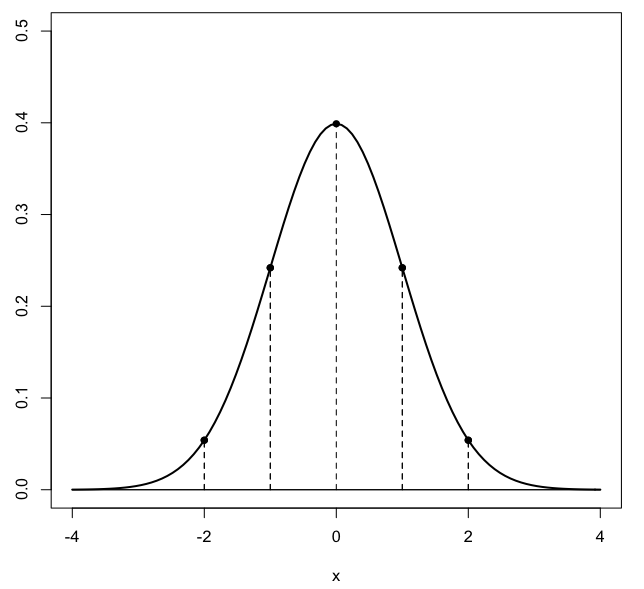
\includegraphics [scale=0.4] {gauss3.png} \end{center}
\begin{document}
\maketitle
\Large
For a function $f(x,y)$, if $f_x = f_y = 0$ when evaluated at some point $P = (x_0,y_0)$, then we are at a \emph{critical point} of $f$, which may be a maximum, a minimum, or neither.

One (sophisticated) way to see that $(x_0,y_0)$ is a critical point of $f$ is to consider the slopes of cross-sections of the surface.  If we take the cross-section of the surface in the direction where $y$ is constant, that slope is $f_x$, and similarly, when $x$ is constant, we have $f_y$.

Two vectors in these directions are $\mathbf{u} = <1,0,f_x>$, and $\mathbf{v} = <0,1,f_y>$.  At any point on the surface the normal vector perpendicular to both $\mathbf{u}$ and $\mathbf{v}$ is
\[ \mathbf{n} = \mathbf{u} \times \mathbf{v} = <-f_x,-f_y,1> \]
If for some $(x_0,y_0)$, $f_x = f_y = 0$ then $\mathbf{n} = <0,0,1>$.  The normal points straight up, so the tangent plane is horizontal.  This could be a minimum or a maximum of the function.
\subsection*{example}
Verify that $f(x,y) = x^2 + y^2$ has a minimum at $(0,0)$.  By considering the cross-sections where $x=0$ and $y=0$ we can see that those curves are both parabolas opening up, so we have a \emph{paraboloid}.  The surface has radial symmetry, and for each value of $z > 0$, $z = x^2 + y^2$ is a constant, forming a circle.
\[ f_x = 2x, \ \ \  f_y = 2y, \]
These are both zero only at $(0,0)$, which is a critical point.

This function has continuous second derivatives
\[ f_{xx} = 2, \ \ \ f_{yy} = 2, \ \ \, f_{xy} = f_{yx} = 0 \]
The second derivative test says to compute
\[ D = f_{xx}  f_{yy} -  (f_{xy})^2  \]
If $D > 0$ and $f_{xx} > 0$, then the given point is a minimum.

Going through the same arguments for $f(x,y) = -(x^2 + y^2)$, we obtain that $D > 0$ and $f_{xx} < 0$, so the point $(0,0)$ is a maximum.
\subsection*{example}
An alternative surface is given by $f(x,y) = x^2 - y^2$.  By considering the cross-sections where $x=0$ and $y=0$ we can see that both curves are parabolas, but one opens up and the other down.  This is called a \emph{hyperbolic paraboloid}.

In this case
\[ f_x = 2x, \ \ \  f_y = -2y, \]
Again, the only critical point is $(x_0,y_0) = (0,0)$
\[ f_{xx} = 2, \ \ \ f_{yy} = -2, \ \ \, f_{xy} = f_{yx} = 0 \]
\[ D = f_{xx}  f_{yy} -  (f_{xy})^2  < 0 \]
In this case, the point is a \emph{saddle point}.

It might be interesting to look at some more unusual surfaces including the \emph{volcano}
\[ z = (x^2 + y^2) e^{-x^2 + y^2} \]
and the \emph{sombrero}
\[ z = \frac{\sin \pi r}{\pi r} \]
but maybe that's enough for now

\subsection*{example}
Find the minimum distance from the origin to a point on the plane $x + y + z = 3$.

We must minimize the distance
\[ d = \sqrt{x^2 + y^2 + z^2} \]
or, to make things simpler, we minimize the square of the distance (since the distance then will be a minimum as well).
\[ d^2 = x^2 + y^2 + z^2 \]
Substituting for $z$
\[ f(x,y) = d^2 = x^2 + y^2 + (3 - x - y)^2 \]
\[ = x^2 + y^2 + 9 - 3x - 3y - 3x + x^2 + xy - 3y + xy + y^2 \]
\[ = 2x^2 + 2y^2 - 6x - 6y + 2 xy + 9 \]
From the geometry it is clear that there is a single critical point and it is a minimum:
\[ f_x = 4x - 6 + 2y = 0 \]
\[ f_y = 4y - 6 + 2x = 0 \]
Multiply the first equation by $-2$ and add to the second:
\[ -6x + 6 = 0 \]
\[ x = 1 \]
Substitute for $x$ in either equation:
\[ y = 1 \]
Substitute $x = y = 1$ into the equation of the plane:
\[ 1 + 1 + z = 3 \]
\[ z = 1 \]
Note that, of course, the shortest distance of a point to a plane is obtained by moving along the normal vector to the plane, which is indeed $<1,1,1>$.

\subsection*{example}
Find the minimum distance from the point $(1,2,0)$ to the cone $z^2 = x^2 + y^2$.

For any point $(x,y,z)$ in space the square of the distance to $(1,2,0)$ is
\[ d^2 = (x-1)^2 + (y-2)^2 + (z-0)^2 \]
\[ = x^2 - 2x + 1 + y^2 - 4y + 4 + z^2 \]
Use the constraint that the point must lie on the cone:
\[ z^2 = x^2 + y^2 \]
so
\[ d^2 = x^2 - 2x + 1 + y^2 - 4y + 4 + x^2 + y^2 \]
\[ = 2x^2 + 2y^2 -2x -4y + 5 \]
The first derivatives:
\[ f_x = 4x - 2 = 0 \]
\[ f_y = 4y - 4 = 0 \]
Hence
\[ x = \frac{1}{2}, \ \ \ y = 1 \]
\[ z^2 = x^2 + y^2 = \frac{5}{4} \]
The distance is
\[ d = \sqrt{(\frac{1}{2} - 1)^2 + (1-2)^2 + (\frac{5}{4})^2 } \]
which is about $1.58$.

\subsection*{example}
A rectangular box, open at the top is to hold some constant volume $V$ of cat food.  Find the dimensions for which the surface area is a minimum.

Let $x$ and $y$ be the lengths of the sides of the base.  Then the height is
\[ z = \frac{V}{xy} \]
Two sides have area
\[ xz = \frac{V}{x} \]
Two have area 
\[ yz = \frac{V}{y} \]
and the bottom has area $xy$ so the total surface area is
\[ A = \frac{2V}{x} + \frac{2V}{y} + xy \]
we must have
\[ A_x = -\frac{2V}{x^2}  + y = 0 \]
\[ A_y = -\frac{2V}{y^2}  + x = 0 \]
Rearranging the first equation:
\[ y = \frac{2V}{x^2} \]
\[ \frac{1}{y^2} = \frac{x^4}{4V^2} \]
Substitute into the second:
\[ -\frac{x^4}{2V} + x = 0 \]
\[ \frac{x^4}{2V} = x \]
One root is $x=0$ which we discard because that is not a relevant solution.  So
\[ \frac{x^3}{2V} = 1 \]
So 
\[ x = (2V)^{1/3} \]
Now you can go back and solve the same equations for $y$ but I just note that the equations are symmetric in $x$ and $y$ so $x = y$.  The area of the base is then
\[ A = xy = (2V)^{2/3} \]
and the height is
\[ h = \frac{V}{A} =  \frac{V}{(2V)^{2/3}} =  2^{-2/3} V^{1/3} \]
This looks a little weird but if we form the ratio
\[ \frac{h}{x} = \frac{2^{-2/3} V^{1/3}}{ (2V)^{1/3}} = 2^{-1} = \frac{1}{2}  \]
The height is one-half either of the sides.

\end{document}  